% Mars Mission AI - TikZ Architecture Diagrams
% Compile with: pdflatex tikz_diagrams.tex

\documentclass[tikz,border=10pt]{standalone}
\usepackage{tikz}
\usetikzlibrary{shapes.geometric, arrows.meta, positioning, fit, backgrounds, shadows, calc}

\begin{document}

% Define colors
\definecolor{planning}{RGB}{74,144,226}
\definecolor{vision}{RGB}{80,200,120}
\definecolor{marl}{RGB}{255,107,107}
\definecolor{data}{RGB}{255,217,61}
\definecolor{gateway}{RGB}{0,117,143}
\definecolor{database}{RGB}{108,117,125}

% Define styles
\tikzstyle{service} = [rectangle, rounded corners, minimum width=3cm, minimum height=1cm, text centered, draw=black, fill=blue!30, drop shadow]
\tikzstyle{database} = [cylinder, shape border rotate=90, aspect=0.25, minimum width=2.5cm, minimum height=1.2cm, text centered, draw=black, fill=database!30, drop shadow]
\tikzstyle{client} = [rectangle, rounded corners, minimum width=2.5cm, minimum height=1cm, text centered, draw=black, fill=gray!20, drop shadow]
\tikzstyle{arrow} = [thick,->,>=Stealth]
\tikzstyle{bidiarrow} = [thick,<->,>=Stealth]

% ===================================================================
% DIAGRAM 1: High-Level System Architecture
% ===================================================================
\begin{tikzpicture}[node distance=2cm]

% Title
\node[font=\Large\bfseries] at (0,10) {Mars Mission AI - High-Level Architecture};

% Client Layer
\node (client) [client] at (0,8) {Client Applications};

% Gateway Layer
\node (gateway) [service, fill=gateway!30, below=1.5cm of client] {Kong API Gateway\\Port 8000/8001};

% Microservices Layer
\node (planning) [service, fill=planning!30, below left=2cm and 3cm of gateway] {Planning Service\\Port 8005};
\node (vision) [service, fill=vision!30, below=2cm of gateway] {Vision Service\\Port 8002};
\node (marl) [service, fill=marl!30, below right=2cm and 1cm of gateway] {MARL Service\\Port 8003};
\node (dataserv) [service, fill=data!30, below right=2cm and 3cm of gateway] {Data Integration\\Port 8004};

% Data Layer
\node (postgres) [database, below left=3cm and 1cm of planning] {PostgreSQL\\Port 5432};
\node (redis) [database, below right=3cm and 1cm of dataserv] {Redis Cache\\Port 6379};

% ML Models
\node (segformer) [rectangle, rounded corners, minimum width=2cm, minimum height=0.8cm, draw=black, fill=orange!30, below=1.5cm of vision] {SegFormer\\Model};
\node (agents) [rectangle, rounded corners, minimum width=2cm, minimum height=0.8cm, draw=black, fill=red!30, below=1.5cm of marl] {5 RL Agents\\Trained};

% Connections
\draw [arrow] (client) -- (gateway);
\draw [arrow] (gateway) -- (planning);
\draw [arrow] (gateway) -- (vision);
\draw [arrow] (gateway) -- (marl);
\draw [arrow] (gateway) -- (dataserv);

\draw [arrow] (planning) -- (vision);
\draw [arrow] (planning) -- (marl);
\draw [arrow] (planning) -- (dataserv);

\draw [arrow] (vision) -- (segformer);
\draw [arrow] (marl) -- (agents);

\draw [arrow] (dataserv) -- (postgres);
\draw [arrow] (dataserv) -- (redis);
\draw [arrow] (planning) -- (postgres);

% Background boxes
\begin{scope}[on background layer]
    \node[draw=black!50, fill=blue!5, fit=(planning)(vision)(marl)(dataserv), inner sep=0.5cm, rounded corners, label=above:Microservices Layer] {};
    \node[draw=black!50, fill=gray!5, fit=(postgres)(redis), inner sep=0.5cm, rounded corners, label=above:Data Layer] {};
    \node[draw=black!50, fill=yellow!5, fit=(segformer)(agents), inner sep=0.5cm, rounded corners, label=above:ML Models] {};
\end{scope}

\end{tikzpicture}

\newpage

% ===================================================================
% DIAGRAM 2: MARL System Architecture
% ===================================================================
\begin{tikzpicture}[node distance=1.5cm]

% Title
\node[font=\Large\bfseries] at (0,10) {MARL System Architecture};

% Mission Input
\node (input) [rectangle, rounded corners, minimum width=2.5cm, minimum height=1cm, draw=black, fill=blue!20] at (-8,7) {Mission\\Parameters};

% Agents
\node (route) [service, fill=marl!30, minimum width=2.5cm, minimum height=0.8cm] at (-8,4) {Route Planner};
\node (power) [service, fill=marl!30, minimum width=2.5cm, minimum height=0.8cm, below=0.5cm of route] {Power Manager};
\node (science) [service, fill=marl!30, minimum width=2.5cm, minimum height=0.8cm, below=0.5cm of power] {Science Agent};
\node (hazard) [service, fill=marl!30, minimum width=2.5cm, minimum height=0.8cm, below=0.5cm of science] {Hazard Avoidance};
\node (strategy) [service, fill=marl!30, minimum width=2.5cm, minimum height=0.8cm, below=0.5cm of hazard] {Strategic Coordinator};

% Coordination
\node (voting) [rectangle, rounded corners, minimum width=2.5cm, minimum height=1.2cm, draw=black, fill=red!30, drop shadow] at (-2,2.5) {Weighted\\Voting};
\node (consensus) [rectangle, rounded corners, minimum width=2.5cm, minimum height=1cm, draw=black, fill=green!30, drop shadow] at (-2,0.5) {Action\\Selection};

% Learning Components
\node (qtable) [rectangle, minimum width=2.5cm, minimum height=1cm, draw=black, fill=blue!30, drop shadow] at (4,4) {Q-Tables};
\node (replay) [rectangle, minimum width=2.5cm, minimum height=1cm, draw=black, fill=yellow!30, drop shadow] at (4,2) {Experience\\Replay};
\node (update) [rectangle, minimum width=2.5cm, minimum height=1cm, draw=black, fill=orange!30, drop shadow] at (4,0) {Q-Learning\\Update};

% Connections
\draw [arrow] (input) -- (route);
\draw [arrow] (input) -- (power);
\draw [arrow] (input) -- (science);
\draw [arrow] (input) -- (hazard);
\draw [arrow] (input) -- (strategy);

\draw [arrow] (route) -- (voting);
\draw [arrow] (power) -- (voting);
\draw [arrow] (science) -- (voting);
\draw [arrow] (hazard) -- (voting);
\draw [arrow] (strategy) -- (voting);

\draw [arrow] (voting) -- (consensus);
\draw [arrow] (consensus) -- (qtable);
\draw [arrow] (consensus) -- (replay);
\draw [arrow] (replay) -- (update);
\draw [arrow] (update) -- (qtable);

% Feedback loop
\draw [arrow, dashed] (qtable) to[out=180,in=90] (route);

% Background boxes
\begin{scope}[on background layer]
    \node[draw=black!50, fill=red!5, fit=(route)(power)(science)(hazard)(strategy), inner sep=0.3cm, rounded corners, label=above:MARL Agents] {};
    \node[draw=black!50, fill=green!5, fit=(voting)(consensus), inner sep=0.3cm, rounded corners, label=above:Coordination] {};
    \node[draw=black!50, fill=blue!5, fit=(qtable)(replay)(update), inner sep=0.3cm, rounded corners, label=above:Learning] {};
\end{scope}

\end{tikzpicture}

\newpage

% ===================================================================
% DIAGRAM 3: Data Flow Sequence
% ===================================================================
\begin{tikzpicture}

% Title
\node[font=\Large\bfseries] at (0,12) {Data Flow Sequence Diagram};

% Actors
\node (client) [rectangle, minimum width=2cm, minimum height=0.8cm, draw=black, fill=gray!30] at (0,10) {Client};
\node (gateway) [rectangle, minimum width=2cm, minimum height=0.8cm, draw=black, fill=gateway!30] at (3,10) {Gateway};
\node (planning) [rectangle, minimum width=2cm, minimum height=0.8cm, draw=black, fill=planning!30] at (6,10) {Planning};
\node (data) [rectangle, minimum width=2cm, minimum height=0.8cm, draw=black, fill=data!30] at (9,10) {Data};
\node (marl) [rectangle, minimum width=2cm, minimum height=0.8cm, draw=black, fill=marl!30] at (12,10) {MARL};

% Lifelines
\draw[dashed] (client) -- (0,0);
\draw[dashed] (gateway) -- (3,0);
\draw[dashed] (planning) -- (6,0);
\draw[dashed] (data) -- (9,0);
\draw[dashed] (marl) -- (12,0);

% Messages
\draw[->,thick] (0,9) -- node[above] {POST /plan} (3,8.5);
\draw[->,thick] (3,8.3) -- node[above] {forward} (6,7.8);
\draw[->,thick] (6,7.5) -- node[above] {GET /integrated} (9,7);
\draw[->,thick,dashed] (9,6.7) -- node[above] {data} (6,6.2);
\draw[->,thick] (6,6) -- node[above] {POST /optimize} (12,5.5);
\draw[->,thick,dashed] (12,5.2) -- node[above] {optimized plan} (6,4.7);
\draw[->,thick,dashed] (6,4.5) -- node[above] {response} (3,4);
\draw[->,thick,dashed] (3,3.8) -- node[above] {result} (0,3.3);

% Annotations
\node[text width=3cm, align=left] at (15,6) {1. Client requests\\2. Gateway routes\\3. Planning gets data\\4. MARL optimizes\\5. Return result};

\end{tikzpicture}

\newpage

% ===================================================================
% DIAGRAM 4: Deployment Architecture
% ===================================================================
\begin{tikzpicture}[node distance=1.5cm]

% Title
\node[font=\Large\bfseries] at (0,11) {Docker Deployment Architecture};

% Network boundary
\draw[thick, dashed, rounded corners] (-10,-2) rectangle (10,9);
\node at (-8,8.5) {\textbf{Docker Network: mars-network}};

% Gateway Layer
\node (kong) [service, fill=gateway!30] at (0,7) {Kong Gateway\\8000, 8001};
\node (kongdb) [database, right=2cm of kong] {Kong\\PostgreSQL};

% Service Layer
\node (vision) [service, fill=vision!30] at (-6,4) {Vision Service\\mars-vision\\:8002};
\node (marl) [service, fill=marl!30] at (-2,4) {MARL Service\\mars-marl\\:8003};
\node (dataint) [service, fill=data!30] at (2,4) {Data Integration\\mars-data\\:8004};
\node (planserv) [service, fill=planning!30] at (6,4) {Planning Service\\mars-planning\\:8005};

% Data Layer
\node (pg) [database] at (-4,0.5) {PostgreSQL\\mars-postgres\\:5432};
\node (redisdb) [database] at (4,0.5) {Redis\\mars-redis\\:6379};

% Volumes
\node (pgvol) [rectangle, minimum width=2cm, minimum height=0.6cm, draw=black, fill=gray!20] at (-6,-1) {postgres\_data};
\node (redisvol) [rectangle, minimum width=2cm, minimum height=0.6cm, draw=black, fill=gray!20] at (-2,-1) {redis\_data};
\node (modelvol) [rectangle, minimum width=2cm, minimum height=0.6cm, draw=black, fill=gray!20] at (2,-1) {models/};

% Connections
\draw[arrow] (kong) -- (vision);
\draw[arrow] (kong) -- (marl);
\draw[arrow] (kong) -- (dataint);
\draw[arrow] (kong) -- (planserv);

\draw[arrow] (planserv) -- (vision);
\draw[arrow] (planserv) -- (marl);
\draw[arrow] (planserv) -- (dataint);

\draw[arrow] (dataint) -- (pg);
\draw[arrow] (dataint) -- (redisdb);

\draw[arrow, dashed] (pg) -- (pgvol);
\draw[arrow, dashed] (redisdb) -- (redisvol);
\draw[arrow, dashed] (vision) -- (modelvol);
\draw[arrow, dashed] (marl) -- (modelvol);

% Background boxes
\begin{scope}[on background layer]
    \node[draw=black!50, fill=blue!5, fit=(kong)(kongdb), inner sep=0.3cm, rounded corners, label=above:Gateway Layer] {};
    \node[draw=black!50, fill=green!5, fit=(vision)(marl)(dataint)(planserv), inner sep=0.3cm, rounded corners, label=above:Service Layer] {};
    \node[draw=black!50, fill=red!5, fit=(pg)(redisdb), inner sep=0.3cm, rounded corners, label=above:Data Layer] {};
    \node[draw=black!50, fill=gray!5, fit=(pgvol)(redisvol)(modelvol), inner sep=0.3cm, rounded corners, label=above:Volumes] {};
\end{scope}

\end{tikzpicture}

\newpage

% ===================================================================
% DIAGRAM 5: MARL State-Action Space
% ===================================================================
\begin{tikzpicture}[node distance=2cm]

% Title
\node[font=\Large\bfseries] at (0,11) {MARL Agent State-Action Space};

% States
\node (init) [circle, draw=black, fill=blue!30, minimum size=1.5cm] at (0,9) {Init};
\node (observe) [rectangle, rounded corners, draw=black, fill=green!30, minimum width=3cm, minimum height=1.2cm, text width=2.8cm, align=center] at (0,6.5) {Observe State\\{\footnotesize lat, lon, battery,\\time, temp, dust,\\targets, sol}};
\node (select) [rectangle, rounded corners, draw=black, fill=yellow!30, minimum width=3cm, minimum height=1.2cm, text width=2.8cm, align=center] at (5,6.5) {Select Action\\{\footnotesize Move, Turn L/R,\\Science, Wait,\\Recharge}};
\node (execute) [rectangle, rounded corners, draw=black, fill=orange!30, minimum width=2.5cm, minimum height=1cm] at (5,4) {Execute\\Action};
\node (update) [rectangle, rounded corners, draw=black, fill=purple!30, minimum width=2.5cm, minimum height=1cm] at (0,4) {Update\\Environment};
\node (reward) [rectangle, rounded corners, draw=black, fill=red!30, minimum width=2.5cm, minimum height=1cm] at (2.5,2) {Receive\\Reward};
\node (store) [rectangle, rounded corners, draw=black, fill=pink!30, minimum width=2.5cm, minimum height=1cm] at (2.5,0) {Store\\Experience};
\node (qupdate) [rectangle, rounded corners, draw=black, fill=cyan!30, minimum width=2.5cm, minimum height=1cm] at (2.5,-2) {Update\\Q-Table};
\node (check) [diamond, draw=black, fill=gray!30, minimum size=1.5cm, aspect=2] at (0,0) {Terminal?};
\node (end) [circle, draw=black, fill=red!30, minimum size=1.5cm] at (-4,0) {End};

% Arrows
\draw[arrow] (init) -- (observe);
\draw[arrow] (observe) -- (select);
\draw[arrow] (select) -- (execute);
\draw[arrow] (execute) -- (reward);
\draw[arrow] (execute) -- (update);
\draw[arrow] (update) -- (reward);
\draw[arrow] (reward) -- (store);
\draw[arrow] (store) -- (qupdate);
\draw[arrow] (qupdate) -- (check);
\draw[arrow] (check) -- node[left] {No} ++(-2,0) |- (observe);
\draw[arrow] (check) -- node[above] {Yes} (end);

\end{tikzpicture}

\newpage

% ===================================================================
% DIAGRAM 6: MARL Training Performance
% ===================================================================
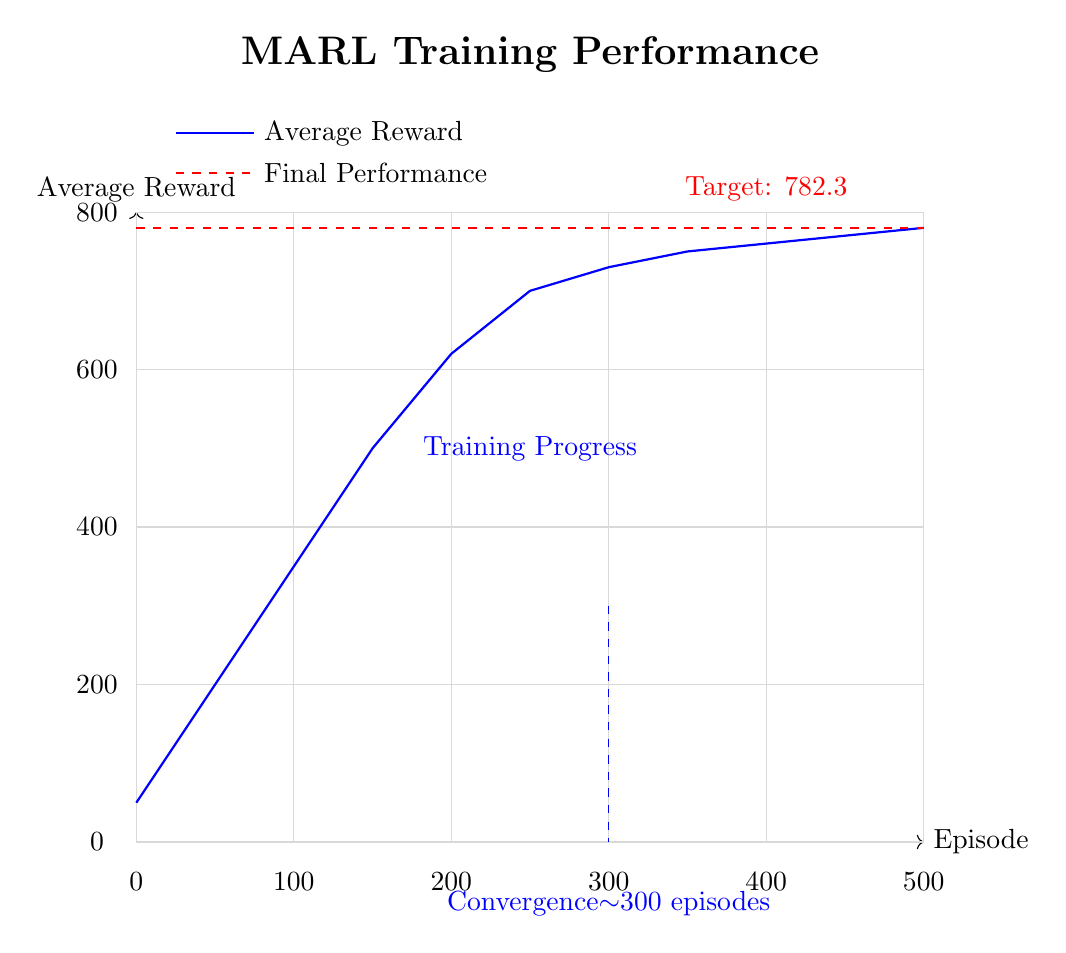
\begin{tikzpicture}

% Title
\node[font=\Large\bfseries] at (5,10) {MARL Training Performance};

% Axes
\draw[->] (0,0) -- (10,0) node[right] {Episode};
\draw[->] (0,0) -- (0,8) node[above] {Average Reward};

% Grid
\foreach \y in {0,2,4,6,8}
    \draw[gray!30] (0,\y) -- (10,\y);
\foreach \x in {0,2,4,6,8,10}
    \draw[gray!30] (\x,0) -- (\x,8);

% Scale labels
\foreach \y in {0,200,400,600,800}
    \node at (-0.5,\y/100) {\y};
\foreach \x in {0,100,200,300,400,500}
    \node at (\x/50,-0.5) {\x};

% Training curve (simplified)
\draw[thick, blue] (0,0.5) -- (1,2) -- (2,3.5) -- (3,5) -- (4,6.2) -- (5,7) -- (6,7.3) -- (7,7.5) -- (8,7.6) -- (9,7.7) -- (10,7.8);

% Convergence line
\draw[thick, red, dashed] (0,7.8) -- (10,7.8);
\node[red] at (8,8.3) {Target: 782.3};

% Annotations
\node[blue] at (5,5) {Training Progress};
\draw[blue, dashed] (6,3) -- (6,0);
\node[blue, below] at (6,-0.5) {Convergence\\$\sim$300 episodes};

% Legend
\draw[thick, blue] (0.5,9) -- (1.5,9);
\node[right] at (1.5,9) {Average Reward};
\draw[thick, red, dashed] (0.5,8.5) -- (1.5,8.5);
\node[right] at (1.5,8.5) {Final Performance};

\end{tikzpicture}

\newpage

% ===================================================================
% DIAGRAM 7: Service Response Times
% ===================================================================
\begin{tikzpicture}

% Title
\node[font=\Large\bfseries] at (5,10) {Service Response Times (P95)};

% Bars
\filldraw[fill=vision!50, draw=black] (1,0) rectangle (2,2);
\filldraw[fill=marl!50, draw=black] (3,0) rectangle (4,0.85);
\filldraw[fill=data!50, draw=black] (5,0) rectangle (6,3.2);
\filldraw[fill=planning!50, draw=black] (7,0) rectangle (8,12);

% Axes
\draw[->] (0,0) -- (9,0) node[right] {Service};
\draw[->] (0,0) -- (0,13) node[above] {Time (ms)};

% Scale
\foreach \y in {0,200,400,600,800,1000,1200}
    \node at (-0.7,\y/100) {\y};

% Labels
\node[below] at (1.5,-0.3) {Vision};
\node[below] at (3.5,-0.3) {MARL};
\node[below] at (5.5,-0.3) {Data};
\node[below] at (7.5,-0.3) {Planning};

% Values
\node[above] at (1.5,2) {200ms};
\node[above] at (3.5,0.85) {85ms};
\node[above] at (5.5,3.2) {320ms};
\node[above] at (7.5,12) {1200ms};

\end{tikzpicture}

\newpage

% ===================================================================
% DIAGRAM 8: Microservices Communication Pattern
% ===================================================================
\begin{tikzpicture}[node distance=2.5cm]

% Title
\node[font=\Large\bfseries] at (0,10) {Microservices Communication Pattern};

% External
\node (user) [rectangle, rounded corners, minimum width=2cm, minimum height=1cm, draw=black, fill=gray!30] at (0,8) {User};

% Gateway
\node (gateway) [service, fill=gateway!30, below=of user] {API Gateway\\Load Balancer};

% Services
\node (s1) [service, fill=vision!30, below left=2cm and 3cm of gateway] {Vision\\Service};
\node (s2) [service, fill=marl!30, below=of gateway] {MARL\\Service};
\node (s3) [service, fill=planning!30, below right=2cm and 3cm of gateway] {Planning\\Service};

% Service Discovery
\node (discovery) [rectangle, minimum width=2.5cm, minimum height=1cm, draw=black, fill=blue!20] at (6,2) {Service\\Discovery\\(DNS)};

% Message Queue (optional)
\node (queue) [rectangle, minimum width=2.5cm, minimum height=1cm, draw=black, fill=yellow!30] at (-6,2) {Message\\Queue\\(Optional)};

% Connections
\draw[bidiarrow] (user) -- node[right] {HTTP/REST} (gateway);
\draw[arrow] (gateway) -- (s1);
\draw[arrow] (gateway) -- (s2);
\draw[arrow] (gateway) -- (s3);

\draw[arrow] (s3) -- (s1);
\draw[arrow] (s3) -- (s2);

\draw[arrow, dashed] (s1) -- (discovery);
\draw[arrow, dashed] (s2) -- (discovery);
\draw[arrow, dashed] (s3) -- (discovery);

\draw[arrow, dashed] (s1) -- (queue);
\draw[arrow, dashed] (s2) -- (queue);

% Annotations
\node[text width=3cm] at (9,6) {\small Synchronous\\REST calls};
\node[text width=3cm] at (-9,2) {\small Async\\messaging};

\end{tikzpicture}

% ===================================================================
% DIAGRAM 9: DQN-Enabled MARL (Double DQN)
% ===================================================================
\newpage
\begin{tikzpicture}[node distance=1.2cm]

\node[font=\Large\bfseries] at (0,9) {DQN-Enabled MARL (Double DQN)};

% Tabular vs DQN
\node (tab) [rectangle, rounded corners, draw=black, fill=blue!15, minimum width=4cm, minimum height=1cm] at (-6,6.5) {Tabular Agents};
\node (dqn) [rectangle, rounded corners, draw=black, fill=purple!15, minimum width=4cm, minimum height=1cm] at (2,6.5) {DQN Agents};

% DQN internals
\node (policy) [rectangle, draw=black, fill=purple!30, minimum width=3cm, minimum height=1cm] at (2,4.5) {Policy Net};
\node (target) [rectangle, draw=black, fill=purple!20, minimum width=3cm, minimum height=1cm] at (6,4.5) {Target Net};
\node (replay) [rectangle, draw=black, fill=yellow!30, minimum width=3cm, minimum height=1cm] at (2,2.8) {Replay Buffer};

\draw[arrow] (policy) -- node[above]{copy $\rightarrow$} (target);
\draw[arrow] (replay) -- (policy);

% Coordination
\node (vote) [rectangle, rounded corners, draw=black, fill=red!30, minimum width=3cm, minimum height=1cm] at (-2,3.5) {Weighted Voting};
\draw[arrow] (tab) -- (vote);
\draw[arrow] (policy) -- (vote);

\node at (-6,2) {\small MARL\ Agents (Q-Table)};
\node at (2,1.5) {\small Double DQN w/ target update};

\end{tikzpicture}

% ===================================================================
% DIAGRAM 10: Multi-Rover Coordination
% ===================================================================
\newpage
\begin{tikzpicture}[node distance=1.2cm]
\node[font=\Large\bfseries] at (0,9) {Multi-Rover Coordination};

\node (coord) [rectangle, rounded corners, draw=black, fill=red!20, minimum width=3.5cm, minimum height=1cm] at (0,6.5) {Fleet Coordinator};
\node (marl) [service, fill=marl!30] at (0,4.8) {MARL System};

\node (r1) [client] at (-6,6.5) {Rover A};
\node (r2) [client] at (-6,5.2) {Rover B};
\node (r3) [client] at (-6,3.9) {Rover C};

\draw[arrow] (r1) -- (coord);
\draw[arrow] (r2) -- (coord);
\draw[arrow] (r3) -- (coord);
\draw[arrow] (coord) -- (marl);
\draw[arrow] (marl) -- ++(0,-1.2) node[below]{\small Joint Actions};

\node[align=left, text width=5cm] at (4,5.2) {\small Conflict resolution:\\- Avoid same target cell\\- Hazard-aware tweak\\- Priority ordering};
\end{tikzpicture}

% ===================================================================
% DIAGRAM 11: Predictive Maintenance Flow
% ===================================================================
\newpage
\begin{tikzpicture}[node distance=1.4cm]
\node[font=\Large\bfseries] at (0,9) {Predictive Maintenance Flow};

\node (tele) [rectangle, rounded corners, draw=black, fill=blue!20, minimum width=3.2cm, minimum height=1cm] at (-6,6.5) {Telemetry};
\node (feat) [rectangle, rounded corners, draw=black, fill=yellow!30, minimum width=3.2cm, minimum height=1cm] at (-2,6.5) {Feature Extractor};
\node (model) [rectangle, rounded corners, draw=black, fill=green!30, minimum width=3.2cm, minimum height=1cm] at (2,6.5) {Maintenance Model};
\node (risk) [rectangle, rounded corners, draw=black, fill=red!30, minimum width=3.2cm, minimum height=1cm] at (6,6.5) {Risk Score};

\draw[arrow] (tele) -- (feat);
\draw[arrow] (feat) -- (model);
\draw[arrow] (model) -- (risk);

\node at (2,4.8) {\small Endpoints: /maintenance/train, /maintenance/predict};
\end{tikzpicture}

% ===================================================================
% DIAGRAM 12: Streaming Telemetry (WebSocket)
% ===================================================================
\newpage
\begin{tikzpicture}[node distance=1.2cm]
\node[font=\Large\bfseries] at (0,9) {Streaming Telemetry (WebSocket)};

\node (pub) [service, fill=data!30] at (-5,6.5) {Data Integration};
\node (ws) [rectangle, rounded corners, draw=black, fill=blue!15, minimum width=4cm, minimum height=1cm] at (0,6.5) {WS /ws/telemetry};
\node (mob) [client] at (5,6.5) {Mobile App};

\draw[arrow] (pub) -- node[above]{POST /publish/telemetry} (ws);
\draw[arrow] (ws) -- node[above]{broadcast} (mob);

\end{tikzpicture}

% ===================================================================
% DIAGRAM 13: Voice Command Flow
% ===================================================================
\newpage
\begin{tikzpicture}[node distance=1.2cm]
\node[font=\Large\bfseries] at (0,9) {Voice Command Flow};

\node (user) [client] at (-6,6.5) {User};
\node (voice) [service, fill=blue!20] at (-2,6.5) {Voice Service};
\node (plan) [service, fill=planning!30] at (2,6.5) {Planning};

\draw[arrow] (user) -- node[above]{\small text/audio} (voice);
\draw[arrow] (voice) -- node[above]{\small POST /plan} (plan);

\end{tikzpicture}

% ===================================================================
% DIAGRAM 14: Federated Learning (FedAvg)
% ===================================================================
\newpage
\begin{tikzpicture}[node distance=1.2cm]
\node[font=\Large\bfseries] at (0,9) {Federated Learning (FedAvg)};

\node (agg) [rectangle, rounded corners, draw=black, fill=green!20, minimum width=3.5cm, minimum height=1cm] at (0,6.5) {Aggregator};
\node (c1) [client] at (-6,7.5) {Rover 1};
\node (c2) [client] at (-6,5.5) {Rover 2};
\node (c3) [client] at (-6,3.5) {Rover 3};

\draw[arrow] (c1) -- node[above]{weights} (agg);
\draw[arrow] (c2) -- (agg);
\draw[arrow] (c3) -- (agg);
\draw[arrow] (agg) -- ++(3,0) node[right]{global model};

\node at (0,4.5) {\small Endpoints: /federated/update, /federated/aggregate};
\end{tikzpicture}

% ===================================================================
% DIAGRAM 15: 3D Terrain Visualization
% ===================================================================
\newpage
\begin{tikzpicture}[node distance=1.2cm]
\node[font=\Large\bfseries] at (0,9) {3D Terrain Visualization};

\node (dem) [rectangle, rounded corners, draw=black, fill=gray!20, minimum width=3.5cm, minimum height=1cm] at (-6,6.5) {DEM (npy/tif)};
\node (svc) [service, fill=blue!20] at (-2,6.5) {Visualization3D Service};
\node (hm) [rectangle, rounded corners, draw=black, fill=yellow!30, minimum width=3.5cm, minimum height=1cm] at (2,6.5) {/heightmap JSON};
\node (web) [client] at (6,6.5) {Three.js Viewer};

\draw[arrow] (dem) -- (svc);
\draw[arrow] (svc) -- (hm);
\draw[arrow] (hm) -- (web);
\end{tikzpicture}

% ===================================================================
% DIAGRAM 16: Long-Term Strategic Planning
% ===================================================================
\newpage
\begin{tikzpicture}[node distance=1.2cm]
\node[font=\Large\bfseries] at (0,9) {Long-Term Strategic Planning};

\node (ctx) [rectangle, rounded corners, draw=black, fill=gray!20, minimum width=3.5cm, minimum height=1cm] at (-6,6.5) {Mission Context};
\node (sp) [service, fill=planning!30] at (-1.5,6.5) {Strategic Planner};
\node (obj) [rectangle, rounded corners, draw=black, fill=green!20, minimum width=4.5cm, minimum height=1cm] at (4,6.5) {Weekly Objectives (90d)};

\draw[arrow] (ctx) -- (sp);
\draw[arrow] (sp) -- (obj);
\end{tikzpicture}

% ===================================================================
% DIAGRAM 17: JPL Export (APGEN/PLEXIL)
% ===================================================================
\newpage
\begin{tikzpicture}[node distance=1.2cm]
\node[font=\Large\bfseries] at (0,9) {JPL Export (APGEN/PLEXIL)};

\node (plan) [rectangle, rounded corners, draw=black, fill=blue!20, minimum width=3.5cm, minimum height=1cm] at (-6,6.5) {Mission Plan JSON};
\node (export) [service, fill=planning!30] at (-1.5,6.5) {Export Endpoint};
\node (apgen) [rectangle, rounded corners, draw=black, fill=yellow!30, minimum width=3.5cm, minimum height=1cm] at (4,7.2) {APGEN Output};
\node (plexil) [rectangle, rounded corners, draw=black, fill=yellow!20, minimum width=3.5cm, minimum height=1cm] at (4,5.8) {PLEXIL Output};

\draw[arrow] (plan) -- (export);
\draw[arrow] (export) -- (apgen);
\draw[arrow] (export) -- (plexil);
\end{tikzpicture}

% ===================================================================
% DIAGRAM 18: Mobile App Architecture
% ===================================================================
\newpage
\begin{tikzpicture}[node distance=1.2cm]
\node[font=\Large\bfseries] at (0,9) {Mobile App Architecture (Expo)};

\node (app) [client] at (-6,6.5) {Expo App};
\node (ws) [rectangle, rounded corners, draw=black, fill=blue!15, minimum width=4cm, minimum height=1cm] at (-1.5,6.5) {WS http://...:8004/ws/telemetry};
\node (api) [service, fill=planning!30] at (4,6.5) {REST APIs};

\draw[arrow] (app) -- (ws);
\draw[arrow] (app) -- (api);

\end{tikzpicture}

\end{document}
